\chapter{Preliminaries}

\section{K\"ahler geometry}

In this section we recall the basics of K\"ahler geometry. We then review some important results on the existence of canonical metrics on compact K\"ahler manifolds. A good reference for the material here is (ref) and (ref).

Let \(X\) denote a compact real manifold of dimension \(2n\). Suppose we have an almost complex structure \(J\) on \(X\), that is an automorphism \(J\) of \(T_\RR X\) such that \(J^2 = - \text{Id}\). Recall that the complexified tangent bundle \(T_\CC X := T_\RR X \otimes \CC\) decomposes via eigenspaces of \(J\):
\[
T_\CC X = T^{1,0} X \oplus T^{0,1} X,
\]
where \(T^{(1,0)} X\) has local generators \(\frac{\partial}{\partial z_i} = \frac{1}{2} \left( \frac{\partial}{\partial x_i}  - \sqrt{-1} \frac{\partial}{\partial y_i}  \right) \), and \(T^{(0,1)} X = \overline{T^{(1,0)} X}\) has local generators \(\frac{\partial}{\partial \bar{z}_i} = \frac{1}{2} \left( \frac{\partial}{\partial x_i}  + \sqrt{-1} \frac{\partial}{\partial y_i}  \right)\).

Recall we have a natural isomorphism of real vector bundles \(T_\RR X \to T^{(1,0)}\), given by the composition \(T_\RR X \to T_\CC \to T^{1,0}X\), and note by definition the action of \(J\) is described by  multiplying by \(\sqrt{-1}\) on \(T^{1,0} X\). The decomposition above induces a decomposition of the complexified cotangent bundle \(T^*_\CC X = T^*_{1,0} X \oplus T^*_{0,1} X\), and moreover a decomposition:
\[
\bigwedge^n T^*_\CC X = \bigoplus_{p+q = n} \left(\bigwedge^p T^*_{1,0} X \otimes \bigwedge^q T^*_{0,1} X   \right)
\]
We will denote \(A^n(X):= H^0(X,\bigwedge^n T^*_\CC X)\) and \(A^{p,q}(X) := H^0 \left( X, \ \left(\bigwedge^p T^*_{1,0} X \otimes \bigwedge^q T^*_{0,1} X   \right) \right) \).

A form \(\alpha \in A^{p,q}(X)\) is said to be \textit{of type \((p,q)\)}. We have the decomposition:
\[
A^n(X) = \bigoplus_{p+q = n} A^{p,q}(X).
\]
A Hermitian metric is given by a smooth choice of positive definite hermitian inner product on the fibers of \(T^{(1,0)}X\), i.e an element of \(H^0(X, T^*_{1,0} X \otimes T^*_{0,1} X) \). Locally we write:
\[
h(z) = \sum h_{ij}(z) dz_i \otimes d\bar{z}_j.
\]

Given a Hermitian metric \(h\) on \(X\), under the isomorphisms \(T_\RR X \cong T^{1,0}X \cong \overline{T^{1,0}X}\) we may consider the real and imaginary parts of \(h\) as real tensors on the underlying real manifold. The real part \(g = \Re h\) is a Riemannian metric on \(X\), called the induced Riemannian metric of \(h\). Locally we have:
\[
g_z = \sum h_{ij}(z) ( dx_i \otimes d x_j + dy_i \otimes dy_j)
\]
We may realize \(\omega = - \Im h\) as an alternating form on the real tangent bundle \(T_\RR X\) via \(T^{1,0}X \cong \overline{T^{1,0}X}\). Set \(\omega ( v \wedge w ) :=  - \Im h(v, \bar{w}) = - \frac{i}{2} ( h - \bar{h} )  \). We call \(\omega\) the associated \((1,1)\)-form of \(h\). Locally we have:
\[
\omega_z = \sqrt{-1} \sum h_{ij}(z) dz_i \wedge d\bar{z}_j = \sqrt{-1} \sum h_{ij}(z) ( dx_i \otimes dy_j - dy_i \otimes dx_j). 
\]
By definition we see \(g(v,w) = g(Jv,Jw)\) and \(\omega(v,w) = g(Jv,w) \) for any \(v,w \in T_\RR X\). In fact we may reconstruct \(h\) from any Riemannian metric \(g\) with \(g(v,w) = g(Jv,Jw)\) or alternatively any real \((1,1)\)-form \(\omega\) satisfying the positive definite condition:
\[
\omega( v \wedge v)  > 0 \text{ for all } v \in T_\RR X.
\]

We may now recall the definition of a K\"ahler manifold.
\begin{definition}
A Hermitian metric is K\"ahler if the associated \((1,1)\)-form \(\omega\) is closed, i.e \(d \omega = 0\) where \(d: A^2(X,\RR) \to A^3(X,\RR)\) is the usual exterior differential.
\end{definition}
We will bow to convention and refer to \(\omega\) as a K\"ahler metric on \(X\) in this context. The standard first example of a compact K\"ahler manifold is complex projective space:
\begin{example}
Consider complex projective space \(\PP^n\). Let \(s\) be a section of the projection map \(\pi: \CC^{n+1} \backslash \{0\} \to \PP^n\) over some open set \(U \subset \PP^n\). The Fubini-Study metric \(\omega_{FS}\) is then defined to be
\[
\omega_{FS} := i \partial \bar{\partial} \log  ||s||^2
\]
This is well-defined as any two sections differ on their shared domain by a non-vanishing holomorphic function, \(s' = fs\). It is clearly closed (since \(d = \partial + \bar{\partial}\)). For the standard section on \(U_0\) with holomorphic coordinates \(z_1,\dots,z_n\) we have:
\[
\omega_{FS} := i \partial \bar{\partial} \log ( 1 + |z_1|^2 + \dots + |z_n|^2)
\]
and at \([1,0,\dots,0] \in U_0\) we have:
\[
\omega_{FS} = i \sum dz_j \wedge d \bar{z}_j
\]
This is positive definite.
\end{example}
\begin{example}
The restriction of \(\omega_{FS}\) to any closed submanifold \(Y \subseteq \PP^n\) produces a K\"ahler structure on \(Y\), as the exterior differential commutes with pulling back differential forms.
\end{example}
\subsection{Line bundles and Kodeira Embedding}
Recall that we can extend the notion of Hermitian metric to an arbitrary complex vector bundle \(E\). A Hermitian metric on \(E\) is an element \(h \in H^0(X, E \otimes \bar{E})^* \).

Recall that a connection is a map
\[
\nabla: H^0(X,E) \to H^0(X,E \otimes T^* X)
\]
satisfying the Liebniz rule \(\nabla(s f) = \nabla s f + s \otimes df\). There is a unique way to extend a connection to and exterior derivative on \(E\)-valued differential forms.
\[
d^\nabla: \Omega^r(E) \to \Omega^{r+1}(E).
\]
The curvature of a connection is the \(2\)-form
\[
F^\nabla \in H^0(X, \text{End}  E \otimes \wedge^2 T^* X),
\]
given by
\[
F^\nabla(u,v)(s) = \nabla_u \nabla_v s - \nabla_v \nabla_u s - \nabla_{[u,v]} s.
\]
There is a canonical connection on the tangent bundle of any Riemannian manifold known as the Levi-Civita connection, satisfying \(\nabla g = 0\) and \(\nabla_u v - \nabla_v u = [u,v]\). We have a similar situation for any Hermitian vector bundle on a complex manifold:	
\begin{example}
Let \(E\) be a Hermitian vector bundle on a complex manifold \(X\) equipped with a holomorphic structure. There is a unique connection \(\nabla\) on \(E\) such that 
\begin{itemize}
\item  \(\pi_{1,0} \nabla s = \bar{\partial} s\)
\item For any smooth vector field \(v\) and smooth sections \(s,t\). \(v \langle s,t \rangle = \langle \nabla_v s , t \rangle + \langle s, \nabla_v t \rangle\) 
\end{itemize}
\end{example}
K\"ahler manifolds may be characterized as those manifolds for which the Levi-Civita connection and Chern connection on the tangent bundle coincide.

We now recall the definition of the first Chern class of a Hermitian line bundle, which may be used to define positivity of curvature. 
\begin{definition}
The first Chern class of a Hermitian line bundle \(L\) is the real cohomology class
\[
c_1(L) = \frac{1}{2 \pi} [  - \sqrt{-1} \partial \bar{\partial} \log(h) ] \in H^2(X, \RR)
\]
\end{definition}
Prop: Every real \((1,1)\)-form in \(c_1(L)\) is the curvature of some Hermitian metric on \(L\).
\begin{example}
Suppose \((X,g)\) is a K\"ahler manifold. Then \(g\) induces a Hermitian metric on the holomorphic cotangent bundle \(\Omega^{1,0} X\), which in turn induces a Hermitian metric on the canonical line bundle \(K_X = \wedge^{n} \Omega^{1,0} X\), denoted \(\det(g)\). The curvature of the associated Chern connection to this Hermitian line bundle is called the Ricci curvature form of the manifold, given by
\[
\Ric(\omega) = - \sqrt{-1} \partial \bar{\partial} \log( \det(g) ).
\]
The real cohomology class \(c_1(K_X) = \frac{1}{2 \pi} [  - \sqrt{-1} \partial \bar{\partial} \log( \det(g) ]  \) is called the first Chern class of the K\"ahler manifold \((X,g)\), and is often denoted just by \(c_1(X)\).
\end{example}
We now recall the definition of a positively curved line bundle.
\begin{definition}
A real \((1,1)\)-form is called positive if the associated symmetric bilinear form defined for real tangent vectors is positive definite. A real cohomology class is called positive if it can be represented by a positive \((1,1)\) form. A line bundle \(L\) is called positive if its first Chern class is positive.
\end{definition}
The following theorem characterizes positive curvature as the same thing as ampleness. Recall that we say \(L\) is very ample if for some global sections \(s_0,\dots,s_n \in H^0(X,L)\) we obtain a well-defined closed embedding into a projective space, given by:
\[
\varphi_L: p \mapsto [s_0(p),\dots,s_n(p)] \in \PP^n
\]
We say \(L\) is ample if some multiple of \(L\) is very ample.
\begin{theorem}[Kodeira Embedding Theorem]
A holomorphic line bundle over a compact complex manifold \(X\) is ample if and only if it is positive.
\end{theorem}
Paired with the following theorem of Chow, this allows us to interchange between talking about compact K\"ahler manifolds and polarized projective algebraic varieties.
\begin{theorem}[Chow Theorem]
A closed complex submanifold of projective space is a projective algebraic subvariety.
\end{theorem}
Now suppose \(X\) is a compact K\"ahler manifold. With example () in mind, either \(K_X = 0\) (etc)
\section{Canonical metrics on K\"ahler manifolds}
As put by Li \cite{li06}, a canonical metric is a choice of metric dependent only on the complex structure of the manifold, and unique up to biholomorphic automorphisms.

Recall the following important result, telling us that any two K\"ahler forms of the same class differ by some real valued function.
\begin{lemma}
If \(\omega, \eta\) are two real \((1,1)\)-forms of the same cohomology class then there is a real function \(f: X \to \RR\) such that \(\omega - \eta = \sqrt{-1} \partial \bar{\partial} f\).
\end{lemma}
\begin{definition}
Let \(X\) be a K\"ahler manifold. A K\"ahler-Einstein metric on \(X\) is a K\"ahler metric \(\omega\) such that \(\Ric \omega = \lambda \omega\) for some real constant \(\lambda\).
\end{definition}
For context we recall the situation in the case of negative and zero Ricci curvature:
\begin{theorem}[Calabi-Yau Theorem]
Let \((X,\omega)\) be a compact K\"ahler manifold. Let \(\alpha\) be a real \((1,1)\)-form representing \(c_1(X)\). Then there exists a real \((1,1)\)-form \(\omega'\) with \([\omega'] = [\omega]\) such that \(\Ric(\omega) = 2 \pi \alpha \)
\end{theorem}
\begin{theorem}[Aubin-Yau]
Let \(X\) be a compact K\"ahler manifold with \(c_1(X) < 0 \). Then there exists a unique K\"ahler metric \(\omega \in -2 \pi c_1(X)\) such that \(\Ric(\omega) = -\omega\).
\end{theorem}
However the following counterexample (Tian) shows us we cannot expect as much in the Fano case.
\begin{example}

\end{example}
In fact the following theorem was also known, giving us a necessary condition for a K\"ahler-Einstein metric.
\begin{theorem}
Matsushima
\end{theorem}
We now introduce the most general form of canonical metric we will consider. This matches the definition given in (Datar and Szekylehidi)
\begin{definition} \label{def:tKRS}
A twisted K\"ahler-Ricci soliton on a Fano manifold \((X,\omega_0)\) is a triple \((\omega,v, t)\) where \(\omega \in 2 \pi c_1(X)\) is a K\"ahler metric, \(v\) is a holomorphic vector field, and \(t \in [0,1]\), such that
\[
\Ric(\omega) - \mathcal{L}_v \omega = t \omega + (1-t) \omega_0
\]
When \(t = 0\) we omit it from the notation and call \((\omega,v)\) a K\"ahler-Ricci soliton. Similarly when \(v\) is trivial we call \((\omega,t)\) a twisted K\"ahler-Einstein metric. When both hold then we talk about \(\omega\) being a K\"ahler-Einstein metric as usual.
\end{definition}
As mentioned in the introduction, K\"ahler-Ricci solitons may be seen as a generalization of K\"ahler-Einstein metrics as they are more general forms of fixed points under the K\"ahler-Ricci flow. The twisted versions of K\"ahler-Einstein metrics and K\"ahler-Ricci solitons originates from the continuity path approach to the respective existence problems.

In chapter () we will see various criteria for the existence of such metrics in an equivariant setting, but first we must recall some basic tools and language from algebraic geometry.
\section{Tools from algebraic geometry} \label{basics}
In this chapter we recall some definitions as we will be understanding them in this thesis.
\subsection{The algebraic torus}
Fix an algebraic torus \(T = (\CC^*)^k\). We have mutually dual character and cocharacter lattices \(M := \Hom(T,\CC^*), \ N = \Hom(\CC^*,N)\) respectively. We denote by \(M_\mathbb{K} := M \otimes_\ZZ \mathbb{K}, \ N_\mathbb{K} := N \otimes_\ZZ \mathbb{K} \) the associated vector spaces, for \(\mathbb{K} = \QQ, \RR\). There is a perfect pairing \(M \times N \to \ZZ\) which extends to a bilinear pairing \(M_\mathbb{K} \times N_\mathbb{K} \to \mathbb{K}\). We often make the identification \( T \cong \spec \CC[M] \cong N \otimes \CC^*. \) Additionally we may identify the real Lie algebra \(\mathfrak{k}\) of the maximal compact subtorus \(K \subset T\) as \( N_\RR = N \otimes \RR.\)
\subsection{Linearizations} \label{basics:linearizations}
\begin{definition}
 Let \(X\) be a projective scheme together with an action \( \lambda : G \times X \to X\) of a reductive algebraic group \(G\). A linearization of the action \(\lambda\) on \(L\) is an action \(\tilde{\lambda}\) on \(L\) such that:
\begin{itemize}
\item The projection \(\pi\) is \(G\)-equivariant, \(\pi \circ \tilde{\lambda} = \lambda \circ \pi \)
\item For \(g \in G\) and \(x \in X\), the induced map \(L_x \mapsto L_{g \cdot x}\) is linear.
\end{itemize}
\end{definition}
%
%
%
Note a linearization to \(L\) naturally induces linearizations to \(L^\vee\) and \(L^{\otimes r}\) for \(r \in \mathbb{N}\).
%
%
%
\begin{example}
A linearization of the trivial bundle on a projective variety \(X\) must be of the form
\[
g \cdot (x,z) = (g \cdot x, \chi(x,z)z)
\]
for some \(\chi \in H^0(G \times X, \mathcal{O}_{G \times X}^*) \cong H^0(G, \mathcal{O}_G^*) = \mathfrak{X}(G).\)
\end{example}
The above example tells us that any two linearizations \(\lambda_1,\lambda_2\) of an action to the same line bundle differ by multiplication by some character \(\chi\) of \(G\): fiberwise we have \(\tilde{\lambda}_1 = \chi(x,z) \tilde{\lambda}_2\). When \(G \cong T\) is an algebraic torus we may identify the set of linearizations with the character lattice \(M\).
\begin{example}
Recall that an action of \(G\) on \(X\) induces a canonical linearization on the tangent and cotangent bundles of \(X\), and so induces a canonical linearization on the anti-canonical bundle \(-K_X\) as the top exterior power of the cotangent bundle.
\end{example}
\subsection{Hamiltonian actions and moment maps} \label{basics:momentmaps}
Here we recall some basic notions of Hamiltonian actions and moment maps. We will follow conventions of \cite{da2006symplectic} and \cite{berman2014complex}. We illustrate the theory with relevant examples of algebraic torus actions. Let \((X,\omega)\) be a real symplectic manifold.
\begin{definition}
Let \(\theta: X \to \RR\) be a smooth function. A vector field \(v\) such that  \(\iota_v \omega = d \theta\) is a hamiltonian vector field with hamiltonian function \(\theta\). 
\end{definition}
\begin{definition}
Let \(K\) be a real Lie group, with Lie algebra \(\mathfrak{k}\), acting smoothly on \(X\). This action is said to be Hamiltonian if there exists a map \(\mu: X \to \mathfrak{k}^*\) such that:
\begin{itemize}
\item For any \(\xi \in \mathfrak{k}\) the map \(\mu^\xi : X \to \RR\) given by \(\mu^\xi(p) := \langle \mu(p), \xi \rangle \) is a hamiltonian function for the vector field \(v\) generated by the one-parameter subgroup \(\exp(t \xi) \subset K\).
\item The map \(\mu\) is equivariant with respect to the action of \(K\) on \(X\) and with respect to the coadjoint action.
\end{itemize}
\end{definition}
Let \(X \subseteq \PP^N\) be a nonsingular complex projective variety and let \(G\) be reductive algebraic group acting effectively on \(\PP^N\), restricting to an action on \(X\). Let \(K\) be the maximal compact subgroup in \(G\), with Lie algebra \(\mathfrak{k}\). The action of \(G\) is given by a representation \(\rho: G \to \text{GL}(N+1)\), and by choosing appropriate coordinates we may assume \(K\) maps to \(U(N+1)\) and so preserves the Fubini-Study form. It can be checked that a moment map \(\mu: X \to \mathfrak{k}^*\) for the \(K\)-action is given by:
\begin{equation}\label{eq:mu}
\mu([x]) \cdot a := \frac{x^t \rho_*(a) \hat{x}}{ |x|^2}
\end{equation}
Where \(x\) is any representative of \([x] \in X \subseteq \PP^N\). This moment map is unique up to translations in \(\mathfrak{k}^*\). A different choice of linearization in this setting corresponds to multiplying \(\rho\) by some character \(\chi \in \mathfrak{X}(G)\).

Since \(\chi(K)\) is compact it sits inside \(S^1 \subset \CC^*\), and hence we do not need to change coordinates when considering the effect on the moment map. When we plug this into (\ref{eq:mu}) we see that we have translated the moment map by \(\chi \in \mathfrak{X}(G) \otimes \RR \cong \mathfrak{k}^*\). Moreover, taking the \(r\)th power of \(L\) corresponds to scaling the moment map by a factor of \(r\). This gives a correspondence between rational elements \(\chi \in \mathfrak{X}(G) \otimes \QQ \subset \mathfrak{k}^*\) and linearizations of powers of \(L\).
\begin{example}
Suppose \(G = T\) is an algebraic torus with character and cocharacter lattices \(M,N\) respectively. Then \(\rho\) is a diagonal matrix of characters \(u_0,\dots,u_{N}\) and we obtain:
\[
\mu([x]) = \frac{\sum_{j=0}^N |x_i|^2 u_i}{|x|^2} \in M
\]
Then, by Atiyah, \cite{atiyah1982convexity}, and Guillemin-Sternberg, \cite{guillemin1982convexity}, the image of \(\mu\) is a convex polytope \(P \subset M\). Here we see that for each one-parameter subgroup \(w \in N\) we have Hamiltonian function
\[
\theta_w([x]) := \langle \mu([x]), w \rangle  
\]
\end{example}
\subsection{Chow and GIT quotients} \label{basics:Chowquotients}
Here we recall the definition of GIT, Chow, and limit quotients of a projective variety by a reductive algebraic group \(G\). We also explain how, when \(G\) is a torus, they may be explicitely calculated via the Kempf-Ness theorem, and recall how GIT quotients behave under smooth blowup.
\subsubsection{GIT quotients}
Recall the basic setup of Mumford's geometric invariant theory, which provides a method for finding geometric quotients on open subsets of a scheme \(X\) when the acting algebraic group \(G\) is reductive. A good reference is \cite{mumford1994}.
%
%
%
In \cite{mumford1994} Mumford introduced the notion of a good categorical quotient, which can be shown to be unique if it exists.
%
%
%
\begin{definition}
A surjective \(G\)-equivariant morphism \(\pi : X \to Y\) is a good categorical quotient if the following hold:
\begin{enumerate}
\item We have \(\mathcal{O}_Y = (\pi_* \mathcal{O}_X)^G\);
\item if \(V\) is a closed \(G\)-invariant subset of \(X\) then \(\pi(V)\) is closed;
\item if \(V,W\) are closed \(G\)-invariant subsets of \(X\) and \(V \cap W = \emptyset\) then we have \(\pi(V) \cap \pi(W) = \emptyset\).
\end{enumerate}
\end{definition}
%
%
%
Good quotients do not always exist for a given scheme \(X\), but we might hope that there exists some dense open subset of \(X\) which does admit a good quotient. Consider the affine case, where \(X = \spec A\). For \(G\) reductive then it can be shown that \(X \sslash G : = \spec A^G\) is a good categorical quotient.

The same ansatz works in the projective case once we make a choice of a lift of the action to the ring of sections of a given ample line bundle. This choice is known as a linearization of the group action.
%
%
%
%
%
%
A linearization \(u\) of a group action \(G\) on \(X\) to \(L\) induces an action of \(G\) on the ring of sections \(R(X,L) := \bigoplus_{j \ge 0} H^0(X,L^{\otimes j}) \). Consider the scheme \(X \sslash_u G := \proj R(X,L)^G\). Note we have a birational map from \(X\) to \(X \sslash_u G\), defined precisely at \(x \in X\) such that there exists some \(m> 0 \) and \(s \in R(X,L)^G_m\) such that \(s(x) \neq 0\). Such a point is said to be semi-stable. If in addition \(G \cdot x\) is closed and the stabilizer \(G_x\) is dimension zero, the point \(x\) is said to be stable. The set of semi-stable and stable points will be denoted by \(X^{ss}(u)\) and \(X^{s}(u)\) respectively.
%
%
%
\begin{construction}[{\cite[Chapter 1, Section 4]{mumford1994}}]
The canonical morphism \(X^{ss}(u) \to X\sslash_u G := \proj R(X,L)^G \) is a good categorical quotient.
\end{construction}
\subsubsection{Kempf-Ness approach to GIT quotients}
One approach to calculating GIT quotients is via the Kempf-Ness theorem. Let \(X \subseteq \PP^N\) be a nonsingular complex projective variety and let \(G\) be reductive algebraic group acting effectively on \(\PP^N\), restricting to an action on \(X\). Let \(K\) be the maximal compact subgroup in \(G\), with Lie algebra \(\mathfrak{k}\). The action of \(G\) is given by a representation \(\rho: G \to \text{GL}(N+1)\), and by choosing appropriate coordinates we may assume \(K\) maps to \(U(N+1)\) and so preserves the Fubini-Study form. It can be checked that a moment map \(\mu: X \to \mathfrak{k}^*\) is given by:
\begin{equation}\label{eq:mu}
\mu([x]) \cdot a := \frac{x^t \rho_*(a) \hat{x}}{ |x|^2}
\end{equation}
Where \(x\) is any representative of \([x] \in X \subseteq \PP^N\). Note we are now in the situation of the previous subsection, with \(L = \mathcal{O}_X(1)\) under the embedding \(X \subseteq \PP^N\). This moment map is unique up to translations in \(\mathfrak{k}^*\). A different choice of linearization in this setting corresponds to multiplying \(\rho\) by some character \(\chi \in \mathfrak{X}(G)\).

Since \(\chi(K)\) is compact it sits inside \(S^1 \subset \CC^*\), and hence we do not need to change coordinates when considering the effect on the moment map. When we plug this into (\ref{eq:mu}) we see that we have translated the moment map by \(\chi \in \mathfrak{X}(G) \otimes \RR \cong \mathfrak{k}^*\). Moreover, taking the \(r\)th power of \(L\) corresponds to scaling the moment map by a factor of \(r\). This gives a correspondence between rational elements \(\chi \in \mathfrak{X}(G) \otimes \QQ \subset \mathfrak{k}^*\) and linearizations of powers of \(L\).
\begin{example}
Suppose \(G = T\) is an algebraic torus with character and cocharacter lattices \(M,N\) respectively. Then \(\rho\) is a diagonal matrix of characters \(u_0,\dots,u_{N}\) and we obtain:
\[
\mu([x]) = \frac{\sum_{j=0}^N |x_i|^2 u_i}{|x|^2} \in M
\]
Then, by Atiyah, \cite{atiyah1982convexity}, and Guillemin-Sternberg, \cite{guillemin1982convexity}, the image of \(\mu\) is a convex polytope \(P \subset M\).
\end{example}
%
%
%
We will make use of the following theorem of Kempf and Ness. A proof is given in \cite[Chapter 8]{mumford1994}. See also the original work \cite{kempf1979}.
\begin{theorem}[{\cite[Theorem 8.3]{kempf1979}}]\label{thm:KN}
Let \(X \subseteq \PP^N\) be a nonsingular complex projective variety and let \(G\) be reductive algebraic group acting effectively on \(\PP^N\), restricting to an action on \(X\). Consider a linearization of some power of \(L\) corresponding to a rational element \(u \in \mathfrak{k}^*\).
\begin{enumerate}
\item \(X^{ss}(u) = \{ x \in X | \overline{Gx} \cap \mu^{-1}(u) \neq \emptyset \} \). \\
\item The inclusion of \(\mu^{-1}(u)\) into \(X^{ss}(u)\) induces a homeomorphism
\[
\mu^{-1}(u)/K \to X\sslash_u G
\]
where \(\mu^{-1}(u)/K\) is endowed with the quotient topology induced from the classical (closed submanifold topology) on \(\mu^{-1}(u)\), and \(X \sslash_u G\) is endowed with its classical (complex manifold) topology
\end{enumerate}
\end{theorem}
%
%
%
We can use Theorem~\ref{thm:KN} to calculate GIT quotients by inspection. To be explicit, suppose \(\mu^{-1}(u)/K\) has the structure of a complex projective variety and \(q: X^{ss}(u) \to \mu^{-1}(u)/K\) is a \(G\)-invariant morphism which restricts to the topological quotient map on the moment fibre, such that \(q_* \mathcal{O}_X^G = \mathcal{O}_Y\). The following fact is probably well known, but we prove it here for the reader's convenience.
\begin{lemma}\label{lem:catquot}
The morphism \(q\) is a good categorical quotient and hence is isomorphic to the GIT quotient map \(X \to X\sslash_u G\).
\end{lemma}
%
%
%
\begin{proof}
It is enough to show that \(q\) sends closed \(G\)-invariant subsets to closed subsets, and disjoint pairs of closed invariant subsets to disjoint pairs of closed subsets.

Firstly suppose that \(V\) is a  \(G\)-invariant Zariski-closed subset of \(X\). Then \(q(V) = q(V \cap \mu^{-1}(u))\), and \(V \cap \mu^{-1}(u)\) is \(K\)-invariant and closed in the classical topology of \(\mu^{-1}(u)\). This implies that \(q(V)\) is closed in the classical topology on \(\mu^{-1}(u)/K \simeq X\sslash_u G\). But \(q(V)\) is constructable, as the image of a Zariski-closed subset of \(X\), and so we may conclude that \(q(V)\) is Zariski-closed in \(\mu^{-1}(u)/K \simeq X\sslash_u G\).

Now suppose \(V,W\) are \(G\)-invariant and Zariski-closed in \(X\), with \(x \in V\) and \(y \in W\) such that \(q(x) = q(y)\). By \ref{thm:KN} we may take \({x'} \in \overline{Gx} \cap \mu^{-1}(u), \ {y'} \in \overline{Gy} \cap \mu^{-1}(u)\) such that \(q({x'}) = q({y'})\). These two points lie in the same \(K\)-orbit. By the \(G\)-invariance of \(V,W\) we have \(V \cap W \neq \emptyset\).
\end{proof}
%
%
%
%
%
%
%Consider the action of an algebraic torus \(T\) on complex projective space \(\PP^n\). Suppose we have some subvariety \(X \subseteq  \PP^n\) invariant under the \(T\) action. As usual we have character and cocharacter lattices \(M,N\) of \(T\). Putting homogeneous coordinates \(z_i\) on \(\PP^n\) suppose the action is given by weight \(u_i \in M\) on \(z_i\). A moment map for this action on \(\PP^n\) is given by
%\[
%[z_0:\dots : z_n] \mapsto \frac{\sum_i |z_i|^2 u_i}{\sum |z_i|^2}
%\]
%Any other moment map differs by a character \(u \in M \). The restriction, \(\mu, \) of this moment map to \(X\) serves as a moment map on \(X\). The image of \(X\) under \(\mu\) is a convex polytope \(P \subset M \).
%\begin{theorem}[ Cohomology of...]
%Take \(u \in M\). If \(x \in \mu^{-1}(u) \) then
%\[
%T \cdot x \cap \mu^{-1}(u) = S \cdot x
%\]
%\end{theorem}
%\begin{theorem}
%\end{theorem}
\subsubsection{GIT quotients under smooth blowup}
Here we recall some results from \cite{kirwan}, which we will use in the proof of Theorem~\ref{thm:KE2}. Let \(G\) be a reductive group acting on \(X\). Let \(L\) be an ample \(G\)-invariant line bundle on \(X\). Fix some linearization of the \(G\)-action to \(L\). Suppose \(V\) be a smooth closed \(G\)-stable subvariety of \(X\). Let \(\pi:W \to X\) be the blow-up of \(X\) along \(V\). The goal is to construct a linear action on \(W\) lifting that on \(X\) and describe the GIT quotient \(W^{ss} \to W \sslash G\) in terms of \(X^{ss} \to  \sslash G\) and \(\pi\).


Set \(L_d = \pi^* L^{\otimes d} \otimes \mathcal{O}(-E)\). For \(d\) sufficiently large this is an ample line bundle on \(W\). Denote the exceptional divisor of \(\pi\) by \(E\). Since \(E \cong \PP(N_{V,X})\) and \(\mathcal{O}(-E)_{|E} \cong \mathcal{O}_{\PP(N_{V,X})}(1)\) then the natural action of \(G\) on \(N_{V,X}\) induces an action on \(\mathcal{O}(-E)_{|E}\). We have \(W \backslash E \cong X \backslash V\) and \(\mathcal{O}(-E)_{|W \backslash E}\) is the trivial line bundle, so admits the product action.

The action of \(G\) on \(L\) lifts to \(\pi^* L^{\otimes d} \), and so we obtain a linear action on \(L_d\). By \cite[]{kirwan} sufficiently large \(d\) we have \(W^{ss} \subset X^{ss}\). There exists a line bundle on \(X \sslash G\) with pullback \(L^{\otimes e}\) for some positive integer \(e\), by \cite{Aubin1976}. Then we have:
\begin{lemma}[ {\cite[Lemma 3.11]{kirwan}}]
If \(d\) is a sufficiently large multiple of \(e\) then the geometric invariant theory quotient \(W \sslash G\) is the blowup of \(X \sslash G\) along the image \(V \sslash G\) of \(V\) in \(X \sslash G\). In particular if \(V \sslash G\) is a divisor on \(X \sslash G\) then \(W \sslash G \cong X \sslash G\).
\end{lemma}
\subsubsection{Chow and limit quotients}
Recall the definition of the Chow quotient, as introduced in \cite{kapranov1993}. If \(G\) is any connected linear algebraic group and \(X\) is a projective \(G\)-variety, then orbit closures of points are generically of the same dimension and degree, and so define points in the corresponding Chow variety. The Chow quotient of the \(G\)-action on \(X\) is the closure of this set of points.

We now recall the definition of the limit quotient, from \cite{mumford1994}. The limit quotient is discussed in detail in \cite{baker2012}. Let \(G\) be a reductive algebraic group, and \(X\) a projective \(G\)-variety. Suppose there are finitely many sets of semi-stable points \(X_1,\dots,X_r\) arising from \(G\)-linearized ample line bundles on \(X\).  Whenever \(X_i \subseteq X_j\) holds, there is a dominant projective morphism \(X_i \sslash G \to X_j \sslash G\) which turns the set of GIT quotients into an inverse system. The associated inverse limit \(Y\) admits a canonical morphism \(\bigcap_{i=1}^r X_i \to Y\). The closure of the image of morphism is the limit quotient.

When \(G\) is an algebraic torus there are indeed finitely many semi-stable loci. Moreover, by \cite[Corollary 2.7]{baker2012}, we may calculate the limit quotient by taking the inverse limit of the subsystem obtained by only considering linearizations of powers of one fixed ample line bundle \(L\).
%
%
%
In \cite[Proposition 2.5]{baker2012} it is shown that the Chow quotient and limit quotient coincide when \(G\) is an algebraic torus.

Let \(X\) be a \(T\)-variety. Let \(\pi:X \dashrightarrow Y\) be the Chow quotient map of \(X\) by its torus action. For any prime divisor \(Z\) on \(Y\), the generic stabilizer on a component of \(\pi^{-1}(Z)\) is a finite abelian group. The maximal order across these components is denoted \(m_Z\). We then obtain a boundary divisor for \(\pi\) given by:
\[
B := \sum_Z \frac{m_Z-1}{m_Z} \cdot Z
\]
We then call the pair \((Y,B)\) the Chow quotient pair of the \(T\)-variety \(X\).
\section{$T$-varieties} \label{prelim:Tvar}
In this section we briefly recall the theory of complex \(T\)-varieties. By a \(T\)-variety we will always mean a normal variety with an effective action of an algebraic torus \(T\). Recall the constructions from (algebraic torus section). Let us fix some definitions. By \textit{polyhedron} we shall mean the intersection of finitely many closed affine halfspaces of \(N_\QQ\). By a \textit{cone} we mean the intersection of finitely many closed linear halfspaces of \(N_\QQ\).
\subsection{Toric varieties}
First, for context, let us recall the toric situation. A cone \(\sigma \subset N_\RR\) has a dual cone \(\sigma^\vee := \{ \}\), and we may construct the normal toric variety \(\spec \CC[\sigma^\vee \cap M]\). Conversely, given a normal affine toric variety \(X\) with algebraic torus \(T\), \(\CC[X]\) is a semigroup subalgebra of \(\CC[M]\) of the form \(\CC[\sigma^\vee \cap M]\) for some strongly convex rational polyhedral cone \(\sigma \subset N_\RR\). We write \(\TV(\sigma,N):= \spec \CC[\sigma^\vee \cap M] \).

Face inclusions of cones correspond to equivariant open embeddings of varieties, and so from a complete fan of cones \(\Sigma\) we may construct a normal toric variety \(X_\Sigma\).
\begin{example}
Consider the toric variety \(\PP^1 \times \PP^1\), with action
\[
(s,t) \cdot ( [x_0,x_1],[y_0,y_1]) := ([sx_0,x_1],[ty_0,y_1])
\]
This is given by the following fan:
\begin{figure}[h]
\centering
  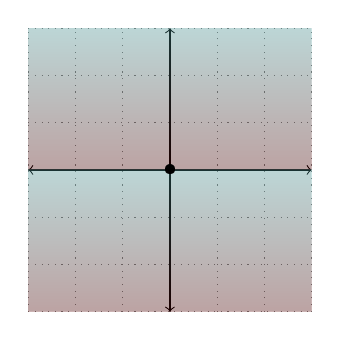
\begin{tikzpicture}[scale=0.6]
   	 \draw[dotted,step=1,gray,] (-3,-3) grid (3,3);
   	 \draw[->] (0,0) -- (0,3);
   	 \draw[->] (0,0) -- (0,-3);
   	 \draw[->] (0,0) -- (3,0);
   	 \draw[->] (0,0) -- (-3,0);
   	 	 \fill[bottom color=red!50!black, top color=cyan!50, opacity=0.2]
  (0,0) -- (3,0) -- (3,3) -- (0,3) -- (0,0);
   	 	 \fill[bottom color=red!50!black, top color=cyan!50, opacity=0.2]
  (0,0) -- (-3,0) -- (-3,3) -- (0,3) -- (0,0);
   	 	 \fill[bottom color=red!50!black, top color=cyan!50, opacity=0.2]
  (0,0) -- (3,0) -- (3,-3) -- (0,-3) -- (0,0);
    	 \fill[bottom color=red!50!black, top color=cyan!50, opacity=0.2]
  (0,0) -- (-3,0) -- (-3,-3) -- (0,-3) -- (0,0);
   	 \draw (0,0) node {\textbullet};
	\end{tikzpicture}
	\caption*{$\Sigma \subset N_\QQ$}
\end{figure}
\end{example}
We recall the combinatorial description of equivariant polarizations of toric varieties via convex polytopes. Suppose we have a complete fan \(\Sigma\), with rays \(\Sigma(1)\). Any Cartier divisor on \(X = \TV(\Sigma)\) is linearly equivalent to a \(T\)-equivariant one, and in summary we have the following exact sequence:
\[
0 \to M \to \cadiv_T(X) \cong \ZZ^{\Sigma(1)} \to \Cl(X) \to 0.
\]
and more explicitely we have the relations \(\div(\chi^u) = \sum_{\rho \in \Sigma(1)} \langle u, v_\rho \rangle D_\rho\).

Recall that to any lattice polytope \(P \subset M_\QQ\) we can associate a normal projective toric variety \(X_P\) given by its dual fan, and an ample divisor \(D_P\) given by coefficients on the ray generators of \(\Sigma(1)\) specified by the equations of halfspaces defining \(P\).
\begin{example}
If we start with \(P\) being the following polytope
\begin{figure}[h]
\centering
  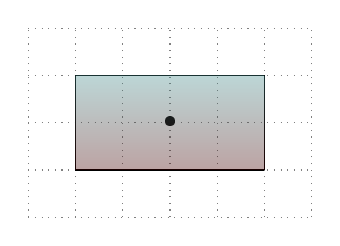
\begin{tikzpicture}[scale=0.6]
   	 \draw[dotted,step=1,gray,] (-3,-2) grid (3,2);
   	 \draw[] (2,-1) -- (2,1) -- (-2,1) -- (-2,-1) -- (2,-1);
   	 \draw (0,0) node {\textbullet};
   	 \fill[bottom color=red!50!black, top color=cyan!50, opacity=0.2]
  (2,-1) -- (2,1) -- (-2,1) -- (-2,-1) -- (2,-1);   	 
	\end{tikzpicture}
	\caption*{$P \subset M_\QQ$}
\end{figure}

Then the normal fan \(\mathcal{N}(P)\) is that of \(\PP^1 \times \PP^1\) as in example (ref). We can calculate the corresponding divisor as
\[
D_P = -2D_{e_1} - D_{e_2} -2 D_{-e_1} - D_{-e_2}  \sim -4 D_{e_1} -2 D_{e_2} 
\]
Where the coefficient at is given by () for example. We see that this divisor represents the line bundle \(\O(4,2)\). (check)
\end{example}
Moreover any equivariant polarization of a toric variety \((X,D)\) may be constructed from some polytope, via the exact sequence (ref).
\subsection{Complexity one $T$-varieties}
There is a successful program to extend the combinatorial dictionary of toric varieties to \(T\)-varieties of higher complexity. Roughly speaking, the combinatorial data lives over the Chow quotient of \(X\) by the \(T\)-action.

Recall that one may define an abelian semigroup structure on the set of all polyhedra via Minkowski addition:
\[
\Delta + \Delta' := \{ v + v' | v \in \Delta, \ v' \in \Delta' \}.
\]
It is well known that this gives a representation of any polyhedron \(\Delta = P + \sigma \) where \(P\) is a convex polytope and \(\sigma\). The cone \(\sigma\) is uniquely specified and is known as the tail cone of \(\Delta\). We will write \(\tail \Delta = \sigma\), and call \(\Delta\) a \(\sigma\)-tailed polyhedra in this situation.

The set of \(\sigma\)-tailed polyhedra form a sub-semigroup \(\Pol_\QQ^+(N,\sigma)\). We also include \(\emptyset\) here, with \(\emptyset + \Delta := \emptyset\) for any \(\Delta\). We may now recall the definition of a polyhedral divisor:
\begin{definition}
Let \(\sigma \subset N_\RR\) be a cone, and \(Y\) a normal projective variety over \(\CC\). A polyhedral divisor on \((Y,N)\) with tail cone \(\sigma\) is an element \(\mathcal{D} \in \Pol_\QQ^+(N,\sigma) \otimes \cadiv_\QQ^+(Y)\), where \(\cadiv_\QQ^+(Y)\) is the semigroup of effective \(\QQ\)-Cartier divisors on \(Y\). We write \(\tail \D = \sigma\).
\end{definition}
Let \(\Loc \D := Y \backslash \bigcup_{\D_Z = \emptyset} Z\). The evaluation of \(\D\) at \(u \in \sigma^\vee\) is defined to be the \(\QQ\)-Cartier divisor on \(Y\) given by:
\[
\D(u) :=  \sum_{\D \neq \emptyset} \min_{v \in \D_P} \langle v,u \rangle Z_{|\Loc \D}.
\]
\begin{definition}
A polyhedral divisor \(\D\), as defined above, is called a \(p\)-divisor if \(\D(u)\) is semiample for \(u \in \sigma^\vee\) and, in addition, big for \(u \in \text{int}(\sigma^\vee)\). Note if \(\Loc \D\) affine this is automatically satisfied.
\end{definition}

By \cite[Proposition 3.1]{hausen2018torus}, \(p\)-divisor defines an affine \(T\)-variety in the following manner. Note for \(u \in \sigma^\vee\) we have \(\D(u) + \D(u') \le \D(u+u')\). Consider the sheaf of \(N\)-graded algebras
\[
\mathcal{A} := \bigoplus_{w \in \sigma^{\vee}} \O_{\Loc \D} (\D(u)).
\]
Define \(\TV(\D) := \spec H^0(\Loc \D, \mathcal{A}) \). Note the semiample and big conditions in the definition of a \(p\)-divisor ensure that the algebra \(H^0(\Loc \D, \A)\) is finitely generated.

The resulting \(T\)-variety \(\TV(\D)\) remains unchanged if we pull back \(\D\) by some birational \(\varphi: Y' \to Y\), i.e if \(\D' := \) then \(\TV(\D') = \TV(\D)\). Moreover, modifying \(\D\) by an element in the image of the natural map
\[
N \otimes_\ZZ \CC(Y)^* \to \Pol_\QQ^+(N,\sigma) \otimes \cadiv_\QQ^+(Y)
\]
also does not change \(\TV(\D)\). Such an element is known as a \textit{principal polyhedral divisor}

In the converse direction, by \cite[Proposition 3.4]{hausen2018torus}, any affine \(T\)-variety \(X\) is of the form \(\TV(\D)\) for some \(p\)-divisor \(\D\). In fact one can define morphisms of \(p\)-divisors, and this correspondence turns out to be an equivlance of categories between affine \(T\)-varieties and \(p\)-divisors up to equivalence via the modifications mentioned above.
\begin{example}
downgrade situation, toric example,
\end{example}

In complexity one, \(Y\) is a curve. Here the degree polyhedron
\[
\deg \D :=
\]
plays an important role. Note the condition (ref) becomes X. Either \(\Loc \)... Therefore any complexity one normal affine \(\T\)-variety may be realized as \(\TV(\D)\) where \(\D\) is a \(p\)-divisor over \(\PP^1\).

By (ref) we have a method of gluing \(p\)-divisors in a natural way to construct general \(T\)-varieties, generalizing the notion of a fan of cones in the toric case. Here we recall the situation in complexity one, where this gluing data is simplified using degree polyhedra, 

By a \textit{complete polyhedral decomposition} we mean a decomposition of \(N_\QQ\) into a collection of polyhedra, closed under intersection. A complete polyhedral decomposition will have a \textit{tail fan}: a fan comprised of exactly the tail cones of the polyhedra in the decomposition. If \(\mathcal{G}\) is a polyhedral decomposition then we write \(\tail \mathcal{G}\) for its tail fan, and for \(\sigma \in \tail \mathcal{G}\) we write  \(\mathcal{G}^\sigma\) for the polyhedron in \(\mathcal{G}\) with tail cone \(\sigma\).

Minkowski addition of polyhedra lifts to the level of complete polyhedral decompositions with a prescribed tail fan. For a given fan \(\Sigma\) denote by \(\PD^+_\QQ(N,\Sigma)\) the corresponding semigroup.

\begin{definition}
A complete \(f\)-divisor is a pair \(\mathcal{S} = \left( \sum_{y \in \PP^1} S_y \otimes \{y\}, \ \deg \mathcal{S} \right)\) where
\[
\sum_{y \in \PP^1} S_y \otimes \{y\} \in \PD^+_\QQ(N,\Sigma) \otimes \cadiv_+(\PP^1)
\] such that for any \(\sigma \in \Sigma\) either \(\sigma \cap \deg \mathcal{S} = \emptyset \) or the polyhedral divisor \(S^\sigma := \sum S_y^\sigma \otimes \{y\}\) is a \(p\)-divisor. We call the finite collection of \(S_y \neq \Sigma\) the non-trivial slices of \(S\).
\end{definition}
\begin{example}
Here we give an example of an \(f\)-divisor describing a complexity one threefold. 
\begin{figure}[h]
\centering


\label{fig:fdivex}
\resizebox{0.9\linewidth}{!}{
\begin{subfigure}[b]{0.30\textwidth}
\centering
  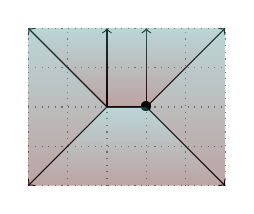
\begin{tikzpicture}[scale=0.5]
   	 \draw[dotted,step=1,gray,] (-3,-2) grid (2,2);
   	 \draw[->] (0,0) -- (0,2);
   	 \draw[] (0,0) -- (-1,0);
   	 \draw[->] (-1,0) -- (-1,2);
   	 \draw[->] (0,0) -- (2,2);
   	 \draw[->] (0,0) -- (2,-2);
   	 \draw[->] (-1,0) -- (-3,2);
   	 \draw[->] (-1,0) -- (-3,-2);
   	 \fill[bottom color=red!50!black, top color=cyan!50, opacity=0.2]
  (0,0) -- (2,-2) -- (2,2) -- (0,0);
   	 \fill[bottom color=red!50!black, top color=cyan!50, opacity=0.2]
  (0,0) -- (2,2) -- (0,2) -- (0,0);
   	 \fill[bottom color=red!50!black, top color=cyan!50, opacity=0.2]
  (0,0) -- (0,2) -- (-1,2) -- (-1,0) -- (0,0);
	 \fill[bottom color=red!50!black, top color=cyan!50, opacity=0.2]
  (-1,0) -- (-1,2) -- (-3,2) -- (-1,0);
  	 \fill[bottom color=red!50!black, top color=cyan!50, opacity=0.2]
  (-1,0) -- (-3,2) -- (-3,-2) -- (-1,0);
   	 \draw (0,0) node {\textbullet};
	 \fill[bottom color=red!50!black, top color=cyan!50, opacity=0.2]
  (0,0) -- (-1,0) -- (-3,-2) -- (2,-2) -- (0,0);
	\end{tikzpicture}
	\caption*{$\mathcal{S}_0$}
\end{subfigure}
\begin{subfigure}[b]{0.30\textwidth}
	\centering
  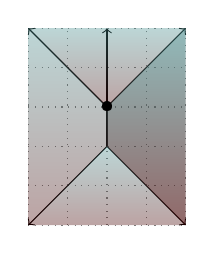
\begin{tikzpicture}[scale=0.5]
   	 \draw[dotted,step=1,gray,] (-2,-3) grid (2,2);
   	 \draw[->] (0,0) -- (0,2);
   	 \draw[] (0,0) -- (0,-1);
   	 \draw[->] (0,0) -- (2,2);
   	 \draw[->] (0,0) -- (-2,2);
   	 \draw[->] (0,-1) -- (2,-3);
   	 \draw[->] (0,-1) -- (-2,-3);
	 \fill[bottom color=red!50!black, top color=cyan!50, opacity=0.2]
  (0,0) -- (0,-1) -- (2,-3) -- (2,2) -- (0,0);
	 \fill[bottom color=red!50!black, top color=cyan!50, opacity=0.2]
  (0,0) -- (2,2) -- (0,2) -- (0,0);
	 \fill[bottom color=red!50!black, top color=cyan!50, opacity=0.2]
  (0,0) -- (0,2) -- (-2,2) -- (0,0);
  	 \fill[bottom color=red!50!black, top color=cyan!50, opacity=0.2]
  (0,0) -- (0,-1) -- (2,-3) -- (2,2) -- (0,0);
  	 \fill[bottom color=red!50!black, top color=cyan!50, opacity=0.2]
  (0,0) -- (-2,2) -- (-2,-3) -- (0,-1) -- (0,0);
  	 \fill[bottom color=red!50!black, top color=cyan!50, opacity=0.2]
  (0,-1) -- (2,-3) -- (-2,-3) -- (0,-1);
   	 \draw (0,0) node {\textbullet};
	\end{tikzpicture}
	\caption*{$\mathcal{S}_1$}
\end{subfigure}
\begin{subfigure}[b]{0.30\textwidth}
	\centering
  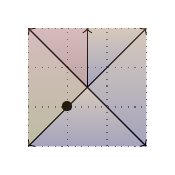
\begin{tikzpicture}[scale=0.5]
   	 \draw[dotted,step=1,gray,] (-1,-1) grid (2,2);
   	 \draw[->] (0.5,0.5) -- (2,2);
   	 \draw[->] (0.5,0.5) -- (0.5,2);
   	 \draw[->] (0.5,0.5) -- (-1,2);
   	 \draw[->] (0.5,0.5) -- (-1,-1);
   	 \draw[->] (0.5,0.5) -- (2,-1);
   	 \draw (0,0) node {\textbullet};
   	           \fill[bottom color=blue!50!black, top color=orange!50, opacity=0.2]
  (0.5,0.5) -- (2,2) -- (2,-1) -- (0.5,0.5);
   	           \fill[bottom color=yellow!50!black, top color=red!50, opacity=0.2]
  (0.5,0.5) -- (-1,2) -- (-1,-1) -- (0.5,0.5);
   	           \fill[bottom color=blue!50!black, top color=orange!50, opacity=0.2]
  (0.5,0.5) -- (2,2) -- (0.5,2) -- (0.5,0.5);
   	           \fill[bottom color=red!50!black, top color=red!50, opacity=0.2]
  (0.5,0.5) -- (-1,2) -- (0.5,2) -- (0.5,0.5);
   	           \fill[bottom color=blue!50!black, top color=orange!50, opacity=0.2]
  (0.5,0.5) -- (2,-1) -- (-1,-1) -- (0.5,0.5);
  
	\end{tikzpicture}
	\caption*{$\mathcal{S}_{\infty}$}
\end{subfigure}
\begin{subfigure}[b]{0.40\textwidth}
	\centering
  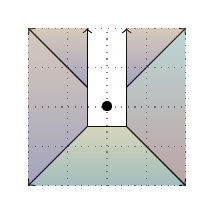
\begin{tikzpicture}[scale=0.5]
   	 \draw[dotted,step=1,gray,] (-2,-2) grid (2,2);
   	 \draw[] (-0.5,-0.5) -- (0.5,-0.5);
   	 \draw[->] (-0.5,-0.5) -- (-0.5,2);
   	 \draw[->] (0.5,-0.5) -- (0.5,2);
   	 \draw[->] (0.5,0.5) -- (2,2);
   	 \draw[->] (-0.5,0.5) -- (-2,2);
   	 \draw[->] (-0.5,-0.5) -- (-2,-2);
  	 \draw[->] (0.5,-0.5) -- (2,-2);
   	 \draw (0,0) node {\textbullet};
   	 \fill[bottom color=red!50!black, top color=cyan!50, opacity=0.2]
  (2,-2) -- (0.5,-0.5) -- (0.5,0.5) -- (2,2) -- (2,-2);
      \fill[bottom color=cyan!50!black, top color=yellow!50, opacity=0.2]
  (2,-2) -- (0.5,-0.5) -- (-0.5,-0.5) -- (-2,-2) -- (2,-2);
      \fill[bottom color=blue!50!black, top color=orange!50, opacity=0.2]
  (-2,-2) -- (-0.5,-0.5) -- (-0.5,0.5) -- (-2,2) -- (-2,-2);
        \fill[bottom color=blue!50!black, top color=orange!50, opacity=0.2]
  (0.5,0.5) -- (0.5,2) -- (2,2) -- (0.5,0.5);
          \fill[bottom color=blue!50!black, top color=orange!50, opacity=0.2]
  (-0.5,0.5) -- (-0.5,2) -- (-2,2) -- (-0.5,0.5);
	\end{tikzpicture}
	\caption*{$\deg \mathcal{S}$}
\end{subfigure}
}
\end{figure}
\end{example}

In complexity one there is a generalization of the correspondence between lattice polytopes and polarized projective toric varieties. We recall the definition of a divisorial polytope, which is used to generalize the polytope description of a polarized toric variety to the complexity one case.
\begin{definition}
A divisorial polytope is a function \(\Psi\) on a lattice polytope \(\Box \subset M_\RR\):
\[
\Psi: \Box \to \wdiv_\RR \PP^1, \ u \mapsto \Sigma_{y \in \PP^1} \Psi_y(u) \cdot \{y\},
\]
such that:
\begin{itemize}
\item For \(y \in \PP^1\) the function \(\Psi_y: \Box \to \RR\) is the minimum of finitely many  affine functions, and \(\Psi_y \equiv 0\) for all but finitely many \(y \in \PP^1\).
\item Each \(\Psi_y\) takes integral values at the vertices of the polyhedral decomposition its regions of affine linearity induce on \(\Box\).
\item \(\deg \Psi(u) > -2\) for \(u \in \text{int} (\Box)\);
\end{itemize}
A divisorial polytope is said to be Fano if additionally we have that:
\begin{itemize}
\item The origin is an interior lattice point of \(\Box\).
\item The affine linear pieces of each  \(\Psi_y\) are of the form \(u \mapsto \frac{\langle v,u \rangle - \beta + 1}{\beta}\) for some primitive lattice element \(v \in N\);
\item Every facet \(F\) of \(\Box\) with \((\deg \circ \Psi _{|F}) \neq -2\) has lattice distance \(1\) from the origin.
\end{itemize}
\end{definition}
Let \(\Psi\) be a divisorial polytope. We may construct a complexity one polarized \(T\)-variety from the graded ring \(S\) given by: 
\[
S_k := \bigoplus_{u \in \Box \cap \frac{1}{k} M} H^0(\PP^1, \mathcal{O}(\lfloor k \cdot ( \Psi(u) +D) \rfloor),
\]
where \(D\) is some integral divisor of degree \(2\). We may also recover a divisorial polytope \(\Psi\) from any polarized complexity one \(T\)-variety \((X,L)\) such that \( H^0(X,L^k) = S_k\). Moreover Fano divisorial polytopes correspond to Fano \(T\)-varieties \((X,-K_X)\). Thus all Fano complexity one \(T\)-varieties may be described in this way. For more details of this construction and the correspondence see \cite{suss2013fano}.

We now recall some basic terminology for divisorial polytopes, which we will make use of in later sections. The push-forward of the measure induced by \(\omega\) is known as the Duistermaat-Heckman measure, independent of the choice of \(\omega\) and which we denote by \(\nu\). Denote the standard measure on \(M_\RR\) by \(\eta\).

\begin{definition}
Let \(\Psi\) be a divisorial polytope.
\begin{itemize}
\item The degree of \(\Psi\) is the map \( \deg \Psi : \Box \to \RR\) given by \( u \mapsto \deg (\Psi(u))\).
\item The barycenter of \(\Psi\) is \(\bc(\Psi) \in \Box\), such that for all \(v \in N_\RR\):
\[
\langle \bc(\Psi), v \rangle = \int_\Box v \cdot \deg \Psi \ d \eta = \int_\Box v d \nu. 
\]
Note by the second equality we see \(\bc(\Psi) = \bc_\nu(\Box).\)
\item The volume of \(\Psi\) is defined to be:
\[
\vol \Psi = \int_\Box \deg \Psi \ d \eta = \int_\Box d \nu.
\]
\end{itemize}
\end{definition}

A Fano divisorial polytope fixes a distinguished representative of \(-K_X\) and specifies a linearisation of the action of \(T\) to \((X,-K_X)\). By the proof of \cite[Theorem 3.21]{petersen2011torus} it is seen that the linearisation coincides with the canonical linearisation of \((X,-K_X)\), and so the moment map specified by the divisorial polytope, with image \(\Box\), coincides with the moment specified by the canonical linearisation.

From here on let \((X,-K_X)\) be the polarized complexity one Fano \(T\)-manifold given by a fixed divisorial polytope \(\Psi: \Box \to \wdiv_\RR \PP^1\), with \(\bc_\nu(\Box) \neq 0\).

\section{Equivariant $K$-stability}
In this section we recall definitions of \(K\)-stability. In summary the \(K\)-stability criteria are concerned with the positivity of certain numerical invariants associated to \textit{test configurations} of our original space. We do not go into detail about how or why \(K\)-stability should relate to the existence of canonical metrics here, but give the definitions and theorems we will rely on later in the thesis.
\subsection{Twisted equivariant $K$-stability}
\label{prelim:twisted}
Here we recall notions of Twisted equivariant $K$-stability, following \cite{datar2016kahler}. Let \(X\) be a Fano manifold with the action of a complex reductive group \(G\) of automorphisms containing a maximal torus \(T\). Fix a \(T\)-invariant K\"ahler form \(\omega \in 2 \pi c_1(X)\) induced by the Fano condition. Recall that the Lie algebra \(\mathfrak{t}\) of the maximal compact torus in \(T\) may be identified with \(N_\RR = N \otimes \RR\).
\begin{definition}
A \(G\)-equivariant test configuration for \((X,L)\) is a \(\CC^*\)-equivariant flat family \(\X\) over the affine line equipped with a relatively ample equivariant \(\QQ\)-line bundle \(\mathcal{L}\) such that:
\begin{enumerate}
\item The \(\CC^*\)-action \(\lambda\) on \((\X, \mathcal{L})\) lifts the standard action on \(\mathbb{A}^1\);
\item The general fiber is isomorphic to \(X\) and \(\mathcal{L}\) is the relative anti-canonical bundle of \(\X \to \mathbb{A}^1\).
\item The action of \(G\) extends to \((\X,\mathcal{L})\) and commutes with the \(\CC^*\)-action \(\lambda\).
\end{enumerate}
A test configuration with \(\X \cong X \times \mathbb{A}^1\) is called a product configuration. If such an isomorphism exists and is \(\CC^*\)-equivariant then we call the test configuration trivial. Finally a test configuration with normal special fiber is called special.
\end{definition}
We work with \(G = T\) being a maximal torus in \(\Aut(X)\). We then have an induced \(T' = T \times \CC^*\)-action on the special fiber. The canonical lift of \(T'\)-action to \(-K_{\X_0}\) induces a canonical choice of moment map \(\mu: \X_0 \to M_\RR'\). The restriction of \(\lambda\) to \(\X_0\) is generated by the imaginary part of a \(T'\)-invariant vector field \(w\), and by an abuse of notation we also write \(w \in N'_\RR\) for the corresponding  one-parameter subgroup. The moment map \(\mu\) then specifies Hamiltonian functions \(\theta_w := \langle \mu, w \rangle: \X_0 \to \RR  \), as we have seen in Section~\ref{basics:momentmaps}.


\begin{definition}
The twisted Donaldson-Futaki character of a special test configuration \((\X, \mathcal{L}) \) is given by:
\[
\DF_{t,\xi}(\X,\mathcal{L},w) = \DF_{\xi}(\X,\mathcal{L},w) + \frac{(1-t)}{V} \int_{\X_0} ( \max_{\X_0} \theta_w - \theta_w)e^{\theta_\xi} \ \omega^n . 
\]
where \(V = \frac{1}{n!} \int_{\X_0} \omega^n\) is the volume of \(\X_0\), and \(\DF_\xi(\X,\L,w) = \frac{1}{V} \int_{\X_0} \theta_w \omega^n\) is the modified Donaldson-Futaki invariant of the configuration, in the form given in \cite[Lemma 3.4]{berman2014complex}.
\end{definition}
\begin{definition}
We say the triple  \((X,t,\xi)\) is \(G\)-equivariantly \(K\)-semistable if \( \DF_{t,\xi}(\X,\mathcal{L},w) \ge 0\) for all \(G\)-equivariant special configurations \((\X,\mathcal{L},w)\). We say \((X,t,\xi)\) is \(K\)-stable if in addition equality holds precisely for product configurations. 
\end{definition}
We will use the following theorem later:
\begin{theorem}[Berman-Witt-Nystrom] \label{thm:BWN}
If \((X,\xi)\) admits a K\"ahler-Ricci soliton then \((X,\xi)\) is \(K\)-stable.
\end{theorem}
From (Datar and Sze) we have a result in the converse direction:
\begin{theorem}[{\cite[Proposition 10]{datar2016kahler}} ] \label{thm:DS}
Let \(X\) be a polarized Fano manifold, with K\"ahler form \(\omega\). Let \(t \in [0,1]\) and \(\xi\) be a soliton candidate for \(X\). Then \((X,t)\) is \(G\)-equivariantly \(K\)-semistable only if for all \(s <t\)  there exists \(\omega_s \in 2 \pi c_1(X)\) such that \(\Ric(\omega_s) - \mathcal{L}_\xi \omega_s = s \omega_s + (1-s) \omega\).
\end{theorem}
\subsection{$K$-stability of $T$-varieties} \label{subsec:IS}
Here we review \(K\)-stability in complexity one. In \cite{ilten2015} Ilten and Suess described non-product special test configurations for a \(T\)-variety of complexity one in terms of its divisorial polytope. We first recall, from \cite{ilten2015}, the description of special fibers of non-product special configurations.

Let \(X\) be a Fano \(T\)-variety of complexity \(1\), corresponding to the Fano divisorial polytope \(\Psi : \Box \to Y\). Without loss of generality we may assume \(Y = \PP^1\). Then there exists some \(y \in \PP^1\), with at most one of \(\Psi_z\) having non-integral slope at any \(u \in \Box\) for \(z \neq y\), such that \(\X_0\) is the toric variety corresponding to the following polytope:
\begin{equation*}
\Delta_y := \Big\{(u,r) \in M_\RR \times \RR \; \Big| \; u \in \Box,\; -1-\sum_{z \neq y} \Psi_z(u) \leq r \leq 1+\Psi_y(u)\Big\}.\label{eq:special-fibre}
\end{equation*}

Furthermore, the induced \(\CC^*\)-action on \(\X_0\) is given by the one-parameter subgroup of 
 \(T' = T \times \CC^*\) corresponding to \(v'=(-mv,m) \in N \times \ZZ\), for some \(v \in N\). In fact it turns out, from \cite{ilten2015}, it is enough to consider those configurations with \(m=1\). As observed in \cite{ilten2015}, we obtain a description of the (non-twisted) Donaldson-Futaki character of $(\X_0,\xi')$:
\begin{equation}
\DF_{\X_0, \xi'}(v') = \frac{1}{\vol \Delta_y}\left(\int_{\Delta_y} \langle u', v' \rangle \cdot e^{\langle u', \xi'\rangle} du'\right),\label{eq:futaki-character}
\end{equation}
with $\xi',v' \in N_\RR \times \RR$. On the other hand, for $v,\xi \in N_\RR$ one obtains:
\begin{equation}
\DF_{X, \xi}(v) = F_{\X_0, (\xi,0)}((v,0))
= \frac{1}{\int_\Box \deg \bar \Phi(u) \,du }\left(\int_{\Box} \langle u, v \rangle \cdot \deg \bar \Phi(u) \cdot e^{\langle u, \xi \rangle}\, du\right)
, \label{eq:futaki-general-fibre}
\end{equation}